
\documentclass[10pt,conference]{IEEEtran}
\usepackage{amsmath,amssymb,amsfonts}
\usepackage{graphicx}
\usepackage{booktabs}
\usepackage{url}
\usepackage{xcolor}
\usepackage{cite}
\usepackage{array}
\usepackage{caption}
\usepackage{placeins}
\graphicspath{{../figures/}}

\title{A Feasibility-Aware HUBO/QUBO Benchmark for UAV Obstacle-Avoidance with Visibility Cost}

\author{\IEEEauthorblockN{Author names to be finalized}
\IEEEauthorblockA{Affiliations to be finalized\\
Email: to be finalized}}

\begin{document}
\maketitle

\begin{abstract}
Quantum-assisted UAV path planning has recently been studied using QAOA-style obstacle-avoidance formulations, but a low-energy binary sample is not necessarily a valid UAV trajectory. This paper presents a feasibility-aware benchmark for a discrete $8\times8$, $L=20$ UAV grid-planning problem with obstacle avoidance, a line-of-sight visibility cost, and a higher-order temporal buffer-risk term. The horizon $L$ denotes discrete planning layers, not physical seconds. The model uses binary variables $x_{t,v}$ indicating whether the UAV occupies cell $v$ at time layer $t$ and forms a HUBO objective with one-hot, start, motion, obstacle, visibility, terminal-goal, and sustained near-obstacle proximity terms. The instance has 1,280 original binary variables and 118,344 polynomial terms, including 4,392 cubic monomials. We compare A*, RRT-best, a QUAV-style QAOA candidate-path selector, native trajectory-level simulated annealing (SA), the classical \texttt{neal} BQM sampler after HUBO-to-QUBO reduction, and an exact CP-SAT/MILP baseline that minimizes the native HUBO soft objective over hard-feasible paths. The CP-SAT solver returns OPTIMAL and certifies that the best observed SA path is globally optimal for the enforced feasible-path objective, with native HUBO energy $-20752.43$, soft cost 247.57, path length 14, six turns, and 85\% visibility. The results do not claim quantum speedup; they show that feasibility-aware decoding, exact baselines, and quadratization accounting are essential for interpreting quantum-compatible UAV planning results.
\end{abstract}

\begin{IEEEkeywords}
HUBO, QUBO, feasibility-aware benchmarking, UAV path planning, obstacle avoidance, visibility-aware planning, MILP, CP-SAT, QAOA, quantum-compatible optimization.
\end{IEEEkeywords}

\section{Introduction}
UAV path planning in cluttered environments requires at least two safety properties: the path must avoid obstacles, and the decoded plan must be executable under the allowed motion model. When perception or tracking is relevant, the planner may also prefer cells with line of sight to the target. Recent quantum-assisted work such as QUAV~\cite{innan2025quav} formulates UAV obstacle-avoidance path planning using QAOA-style optimization and compares against A* and RRT. QUAV is therefore an important closest reference for quantum-assisted UAV navigation. However, a QAOA, annealing, or QUBO solver returns a binary sample, and the sample must be decoded and checked before it can be called a valid path.

This paper studies a deliberately compact grid abstraction so that modeling and solver behavior can be inspected directly. The goal is not to claim quantum speedup on a small static grid. The goal is to define a reproducible HUBO/QUBO-compatible benchmark, separate energy minimization from actual path validity, and compare classical, quantum-inspired, and quantum-compatible solver pathways on the same problem instance.

\subsection{Problem statement and scope}
The planning problem considered here is a static, discrete visibility-aware path-planning abstraction. A UAV must move from a fixed start cell to a fixed target/goal cell through legal grid transitions while avoiding obstacle cells. Visibility is represented as a soft line-of-sight cost from each candidate UAV cell to the fixed target cell. Thus, this paper does not solve continuous quadrotor control, full moving-target tracking, or camera field-of-view control. The abstraction is intentionally small enough that the encoded binary model, decoded paths, feasibility failures, and exact classical baselines can be inspected in detail. The time horizon $L$ is a design parameter giving the number of discrete planning layers. It is not assumed to be seconds unless a physical sampling time $\Delta t$ is separately assigned.

The contributions are as follows. First, we give a complete binary decision-variable formulation for UAV grid planning with obstacle avoidance and a visibility cost. Second, we identify the real source of higher-order structure: a temporal buffer-risk term, not the static line-of-sight cost. Third, we introduce a feasibility-aware evaluation protocol that reports structural feasibility, goal arrival, and full-task success separately. Fourth, we implement a same-platform QUAV-style QAOA candidate-path baseline, clearly not as official QUAV code but as a reproducible reference following the published workflow. Fifth, we add exact CP-SAT and MILP implementations, enabling global comparison against the native HUBO soft objective over hard-feasible paths.

The novelty should be interpreted narrowly. This paper does not introduce a faster planner than A* or CP-SAT, and it does not demonstrate quantum advantage. Its novelty is the feasibility-aware benchmarking layer around a quantum-compatible UAV HUBO/QUBO formulation: the same decoded paths are compared under graph-search, candidate-path QAOA, native trajectory-SA, quadratized BQM sampling, and exact CP-SAT/MILP baselines, with validity and goal arrival separated from energy. This positioning is intentional because, without exact baselines and decoded-path checks, low-energy quantum-compatible samples can be misleading.


\section{Related Work}
\subsection{Classical and visibility-aware UAV planning}
Classical UAV planning spans graph search, sampling-based planning, trajectory optimization, and perception-aware control. A* remains a standard shortest-path reference on discretized maps~\cite{hart1968}, while RRT provides a widely used sampling-based alternative~\cite{lavalle1998}. For target-tracking and perception-aware flight, Chen \emph{et al.} formulate moving-target tracking in cluttered environments~\cite{chen2016}; Hausman \emph{et al.} study occlusion-aware multi-robot 3D tracking~\cite{hausman2016}; Penin \emph{et al.} combine aggressive target tracking with collision and occlusion avoidance~\cite{penin2018}; and Falanga \emph{et al.} incorporate perception objectives into model-predictive control~\cite{falanga2018}. Wang \emph{et al.} extend visibility-constrained tracking to multiple UAVs~\cite{wang2022}, while Masnavi \emph{et al.} derive a real-time multi-convex MPC for occlusion-free target tracking with collision avoidance~\cite{masnavi2022}. These continuous-control works motivate the visibility term used here, but our problem is deliberately a static discrete benchmark rather than a moving-target control formulation.

\subsection{Quantum and QUBO formulations for UAV/drone optimization}
Quantum optimization for routing has developed rapidly; QUBO provides a standard binary optimization representation~\cite{glover2019}, while QAOA is a widely used variational gate-based approach~\cite{farhi2014}. A systematic review by Osaba \emph{et al.} surveys early quantum-routing formulations and highlights recurring issues of encoding size, constraints, and fair classical comparison~\cite{osaba2022review}. Several UAV-specific studies are especially relevant. Huang \emph{et al.} use variational quantum algorithms, including QAOA and VQE, to select collision-avoiding routes for multiple UAVs from predefined alternatives~\cite{huang2022}. Davies and Kalidindi formulate constrained multi-UAV mission planning as MILP and QUBO and study quantum annealing, QAOA, and VQE routes~\cite{davies2024}. Hua \emph{et al.} investigate QUBO-based drone route planning with quantum/digital annealers and compare against Gurobi on wind-influenced urban routing instances~\cite{hua2024}. Tarquini \emph{et al.} compare QUBO formulations of the Drone Delivery Packing Problem under quantum annealing, simulated annealing, and classical global optimization, emphasizing both qubit-reduction opportunities and feasibility/scalability limits~\cite{tarquini2026}.

More recent UAV-specific frameworks move closer to the present setting. Q4DR combines a QAOA clustering stage with annealing-based drone routing under asymmetric costs, forbidden arcs, and charging constraints~\cite{osaba2025q4dr}. QUAV uses QAOA-style optimization for single-UAV obstacle-avoidance path planning and reports both simulation and quantum-hardware experiments; it is the closest prior work to our candidate-path QAOA baseline~\cite{innan2025quav}. Qiu \emph{et al.} formulate multi-target UAV path planning as QUBO and solve it using a coherent Ising machine, providing another direct example of binary optimization for UAV navigation~\cite{qiu2025}. Barbeau \emph{et al.} formulate 1D and 3D target tracking, including obstacle-distance constraints, as constrained quadratic models for quantum annealing~\cite{barbeau2025}. These studies demonstrate multiple quantum-compatible routes for UAV routing, collision avoidance, and tracking, but they optimize different abstractions and generally do not center evaluation on decoded structural feasibility under a common native objective.

\subsection{QUBO path finding, multi-agent planning, and the gap addressed here}
Beyond UAV-specific work, recent multi-agent path-finding studies are relevant to encoding and scalability. Gerlach \emph{et al.} propose an optimal hybrid quantum-classical MAPF method based on branch-and-cut-and-prize with iteratively solved QUBO conflict subproblems~\cite{gerlach2025}. Gonzalez Villasmil proposes a robotics-oriented time-indexed QUBO with BFS-based logical preprocessing, adaptive penalties, and time-window decomposition for multi-robot grid planning~\cite{villasmil2026}. These works reinforce two lessons that directly motivate our benchmark: path-planning encodings can grow rapidly with space-time discretization, and solver outputs must be interpreted relative to hard feasibility and strong classical references.

Among the works reviewed above, we did not find a study that combines the particular ingredients evaluated here: a single-UAV time-indexed HUBO with a static line-of-sight cost, a genuinely cubic sustained near-obstacle temporal term, explicit HUBO-to-QUBO reduction accounting, decoded feasibility/goal/full-success reporting, and an exact CP-SAT/MILP reference evaluated on the same native objective. The contribution is therefore not a new claim of quantum advantage, but a controlled benchmarking framework designed to expose when apparently favorable binary-optimization energies do or do not correspond to executable UAV paths.

\section{Discrete Planning Model}
Let $G=(V,E)$ be an $N\times N$ grid graph. In the experiments $N=8$, $|V|=64$, and time layers are indexed $t=0,\ldots,L-1$ with $L=20$. Each time layer is one discrete trajectory frame; a larger $L$ gives the planner more room for detours or hovering but increases the number of variables linearly. Let $O\subset V$ be the obstacle set, $s\in V$ the start cell, and $g\in V$ the target cell. The permitted next-cell set is
\begin{equation}
\mathcal{N}(u)=\{u\}\cup\{v\in V:(u,v)\in E\},
\end{equation}
where the self-loop represents hovering.

The binary state variable is
\begin{equation}
 x_{t,v}\in\{0,1\},\qquad x_{t,v}=1 \Leftrightarrow \text{the UAV is at cell }v\text{ at time }t.
\end{equation}
A valid binary solution decodes to a trajectory $\pi=(v_0,\ldots,v_{L-1})$ only if exactly one state variable is active at every layer.

Let $\mathrm{LOS}(u,g)$ denote the rasterized Bresenham line cells strictly between $u$ and $g$. The per-cell visibility/occlusion-depth surrogate is
\begin{equation}
 C_{\mathrm{occ}}(u)=|\mathrm{LOS}(u,g)\cap O|.
\end{equation}
A zero value indicates clear line of sight in this grid model. Let $B\subset V\setminus O$ be the set of non-obstacle cells within Chebyshev distance one of an obstacle. Cells in $B$ are legal but risky.

\section{HUBO Formulation}
The total polynomial objective is
\begin{equation}
\begin{split}
H(x) = &H_{\mathrm{uniq}} + H_{\mathrm{start}} + H_{\mathrm{move}} + H_{\mathrm{obs}} \\
&+ H_{\mathrm{occ}} + H_{\mathrm{prox}} + H_{\mathrm{goal}} + H_{\mathrm{term}} .
\end{split}
\end{equation}
The structural terms are
\begin{align}
H_{\mathrm{uniq}} &= \lambda_u \sum_{t=0}^{L-1}\left(\sum_{v\in V} x_{t,v}-1\right)^2,\\
H_{\mathrm{start}} &= \lambda_s(1-x_{0,s}),\\
H_{\mathrm{move}} &= \lambda_m\sum_{t=0}^{L-2}\sum_{u\in V}\sum_{v\notin\mathcal{N}(u)}x_{t,u}x_{t+1,v},\\
H_{\mathrm{obs}} &= \lambda_o\sum_{t=0}^{L-1}\sum_{v\in O}x_{t,v}.
\end{align}
The static visibility cost is linear:
\begin{equation}
H_{\mathrm{occ}}=\lambda_{\mathrm{occ}}\sum_{t=0}^{L-1}\sum_{u\in V}C_{\mathrm{occ}}(u)x_{t,u}.
\end{equation}
The sole cubic term is the sustained-proximity penalty:
\begin{equation}
H_{\mathrm{prox}}=\lambda_p \eta \sum_{t=1}^{L-2}\sum_{u\in B}\sum_{v\in B\cap\mathcal{N}(u)}\sum_{w\in B\cap\mathcal{N}(v)}x_{t-1,u}x_{t,v}x_{t+1,w}.
\end{equation}
Here $\eta=3$. This term penalizes remaining in connected buffer cells for three consecutive layers. Thus the model is genuinely HUBO, but the higher-order degree comes from temporal buffer-risk modeling rather than from static visibility.

The goal terms are
\begin{align}
H_{\mathrm{goal}} &= \lambda_g\sum_{t=0}^{L-1}\sum_{v\in V}\frac{t+1}{L}\|p_v-p_g\|_2x_{t,v},\\
H_{\mathrm{term}} &= \lambda_{\mathrm{term}}\sum_{v\ne g}x_{L-1,v}.
\end{align}
The updated instance uses $\lambda_u=\lambda_s=\lambda_m=\lambda_o=1000$, $\lambda_{\mathrm{occ}}=10$, $\lambda_p=5$, $\lambda_g=8$, $\lambda_{\mathrm{term}}=50$, and $\eta=3$.

\section{Feasibility-Aware Evaluation}
A solver output is not scored only by total HUBO energy. Each binary sample is decoded and checked directly. We report: structural feasibility, meaning one-hot occupancy, correct start, legal transitions, and no obstacle occupancy; goal arrival, meaning $v_{L-1}=g$; and full-task success, meaning both conditions hold for the same decoded sample. Soft cost and native HUBO energy are then interpreted on valid decoded paths.

This distinction is essential for QUBO/BQM and QAOA-style workflows. A sample can have a low reduced-model energy while failing one-hot, motion, obstacle, or target-arrival checks. Such a sample is not a UAV plan. The benchmark therefore reports feasibility rates and representative decoded trajectories, not energy alone.

\section{Solvers and Implementation}
\subsection{A* and RRT Baselines}
A* searches directly on the grid with obstacle avoidance and a heuristic path cost. RRT-best is a randomized grid planner used as a sampling-style reference. These methods return explicit paths and are checked with the same feasibility evaluator. The RRT-best runtime includes 40 fixed-seed trials and best-cost selection.

\subsection{QUAV-Style QAOA Baseline}
QUAV maps UAV path segments to qubits and applies QAOA-style optimization with obstacle-buffer costs. Since no official public code was available in this workflow, we implemented a QUAV-style candidate-path selector following the published algorithmic description. It generates collision-free candidate paths, assigns a QUAV-style geometric cost using length, buffer steps, and turns, and uses a small QAOA-style one-hot selector over the candidates. This baseline is a same-platform reference only, not an exact reproduction of the authors' implementation.

\subsection{Trajectory-Level SA and \texttt{neal}}
Trajectory-level SA searches over cell sequences and evaluates the native HUBO energy directly, including the cubic term. Its proposal operator preserves one-hot occupancy, start, legal motion, and obstacle avoidance by construction. In contrast, \texttt{neal} is a classical BQM simulated-annealing sampler~\cite{neal}. Therefore the HUBO is first reduced to a QUBO/BQM using \texttt{dimod}~\cite{dimod}; cubic monomials require auxiliary-variable quadratization, following the standard reduction principle of Rosenberg~\cite{rosenberg1975}, before sampling.

\subsection{Exact MILP and CP-SAT Baselines}
We added exact optimization baselines in both CP-SAT and MILP form. Both encodings enforce the path constraints directly: exactly one cell per layer, fixed start, final target arrival, obstacle cells forbidden, and legal transitions. Auxiliary binary variables linearize each cubic proximity monomial $y_{tuvw}=x_{t-1,u}x_{t,v}x_{t+1,w}$. The objective minimizes
\begin{equation}
H_{\mathrm{occ}}+H_{\mathrm{prox}}+H_{\mathrm{goal}}+H_{\mathrm{term}}
\end{equation}
over the hard-feasible set. Because all hard constraints are enforced, every feasible solution has the same hard contribution $-\lambda_u L-\lambda_s=-21000$ under the expanded HUBO implementation. The native HUBO energy is therefore this hard constant plus the optimized soft cost. The CP-SAT model uses OR-Tools~\cite{ortools} and the MILP model uses a linear mixed-integer encoding. The CP-SAT run returned OPTIMAL, so its solution is used as the exact baseline in the final table.

\section{Results}
Table~\ref{tab:instance} summarizes the updated instance.
\begin{table}[t]
\caption{Updated main HUBO instance.}
\label{tab:instance}
\centering
\begin{tabular}{lr}
\toprule
Quantity & Value\\
\midrule
Grid size & $8\times 8$\\
Horizon $L$ & 20\\
Original binary variables & 1,280\\
Total polynomial terms & 118,344\\
Linear terms & 1,280\\
Quadratic terms & 112,672\\
Cubic terms & 4,392\\
Obstacles & 6\\
Buffer cells & 24\\
\bottomrule
\end{tabular}
\end{table}





\begin{table}[t]
\centering
\scriptsize
\caption{Unified same-platform comparison. For deterministic or single-output methods, feasibility columns indicate whether the returned path satisfies the condition. For stochastic solvers, feasibility columns report empirical rates over 50 runs/reads.}
\label{tab:unified}
\resizebox{\columnwidth}{!}{%
\begin{tabular}{lccccccccc}
\toprule
Method & Feas. & Goal & Full & Len. & Turns & Buf. & Vis. & HUBO E & Time\\
\midrule
A* & Yes & Yes & Yes & 14 & 7 & 4 & 85.0\% & -20742.26 & 0.028s\\
RRT & Yes & Yes & Yes & 14 & 5 & 4 & 70.0\% & -20700.19 & 0.043s\\
QUAV-QAOA & Yes & Yes & Yes & 14 & 1 & 3 & 80.0\% & -20725.94 & 4.11s\\
CP-SAT exact & Yes & Yes & Yes & 14 & 6 & 4 & 85.0\% & -20752.43 & 1.02s\\
HUBO-SA & 100.0\% & 16.0\% & 16.0\% & 14 & 6 & 4 & 85.0\% & -20752.43 & 1207.26s\\
QUBO/\texttt{neal} & 12.0\% & 8.0\% & 0.0\% & 18 & 12 & 2 & 20.0\% & -20060.47 & 6.15s\\
\bottomrule
\end{tabular}%
}
\end{table}


\subsection{Decoded Optimized Paths}
Fig.~\ref{fig:decoded_paths} shows the actual decoded paths returned by each method on the same map. This figure is important because the numerical table alone does not reveal how the methods use the obstacle-buffer region or why different objectives prefer different routes. A*, RRT-best, QUAV-style QAOA, CP-SAT, and the best full-success SA trajectory all reach the target without collisions. The \texttt{neal} panel shows the best-energy decoded QUBO sample; it is structurally feasible but fails to reach the target, explaining why its full-task success rate is zero.

\begin{figure*}[t]
\centering
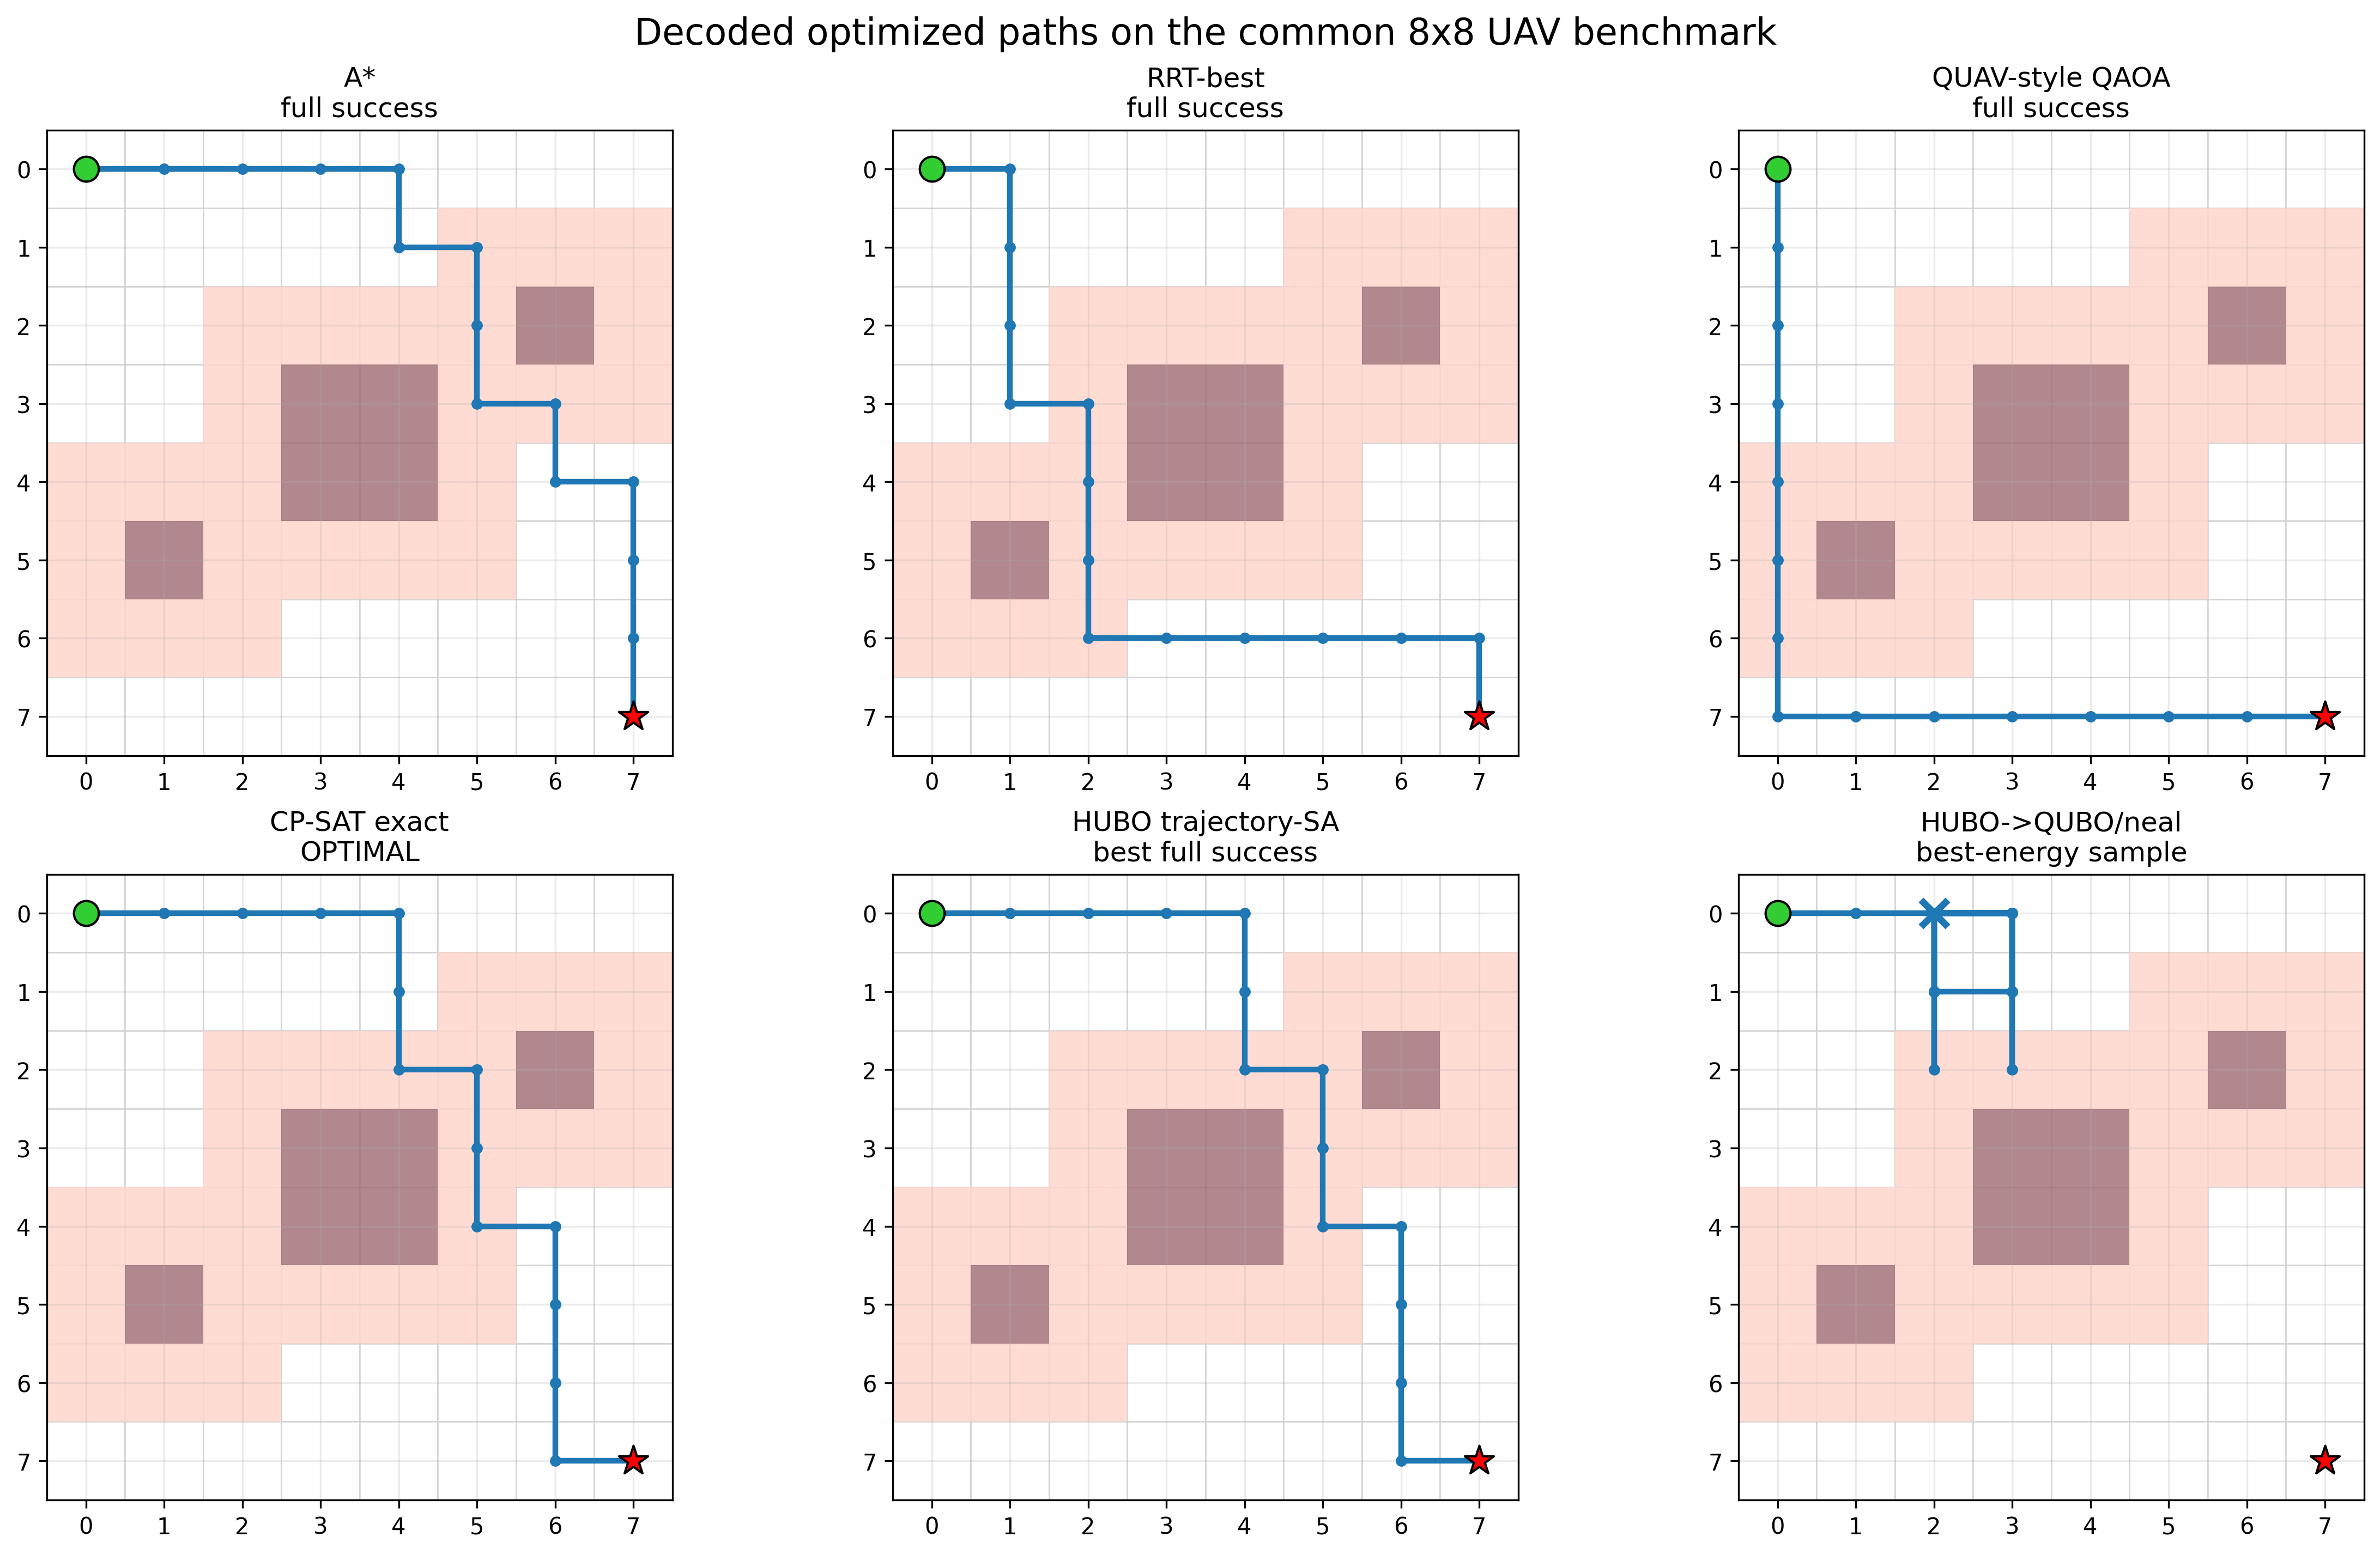
\includegraphics[width=0.98\textwidth]{fig_decoded_paths_all_methods.png}
\caption{Decoded optimized paths on the common $8\times8$, $L=20$ benchmark. Dark cells are obstacles, light cells are obstacle-buffer cells, the green circle is the start, and the red star is the target. The CP-SAT path is globally optimal for the hard-feasible native-HUBO soft objective. The \texttt{neal} path is the best-energy decoded QUBO sample and illustrates a quadratization/sampling failure mode: it is structurally feasible but does not reach the target.}
\label{fig:decoded_paths}
\end{figure*}

The exact CP-SAT baseline reports OPTIMAL, with soft cost 247.57 and native HUBO energy $-20752.43$ in 1.02 s. This matches the best trajectory-SA energy, showing that SA found a globally optimal path for the hard-feasible exact objective on this instance, but SA required 1207.26 s over 50 runs and reached the target in only 8 of 50 runs. A* is much faster and fully successful, but its native HUBO energy is slightly worse because it optimizes a graph-search surrogate rather than the exact cubic proximity-aware objective.

The QUAV-style QAOA selector produces a valid shortest path with only one turn and the lowest QUAV-style geometric cost among its candidates. However, under the native HUBO objective its energy is $-20725.94$, worse than the CP-SAT/SA optimum. This illustrates a central point: a QUAV-style geometric objective and the native HUBO objective are not the same, even when both return collision-free paths. \texttt{neal} after quadratization remains the weakest method in this run: it has 6/50 structural feasibility and 4/50 goal arrival, but 0/50 full-task success.

\begin{figure}[t]
\centering
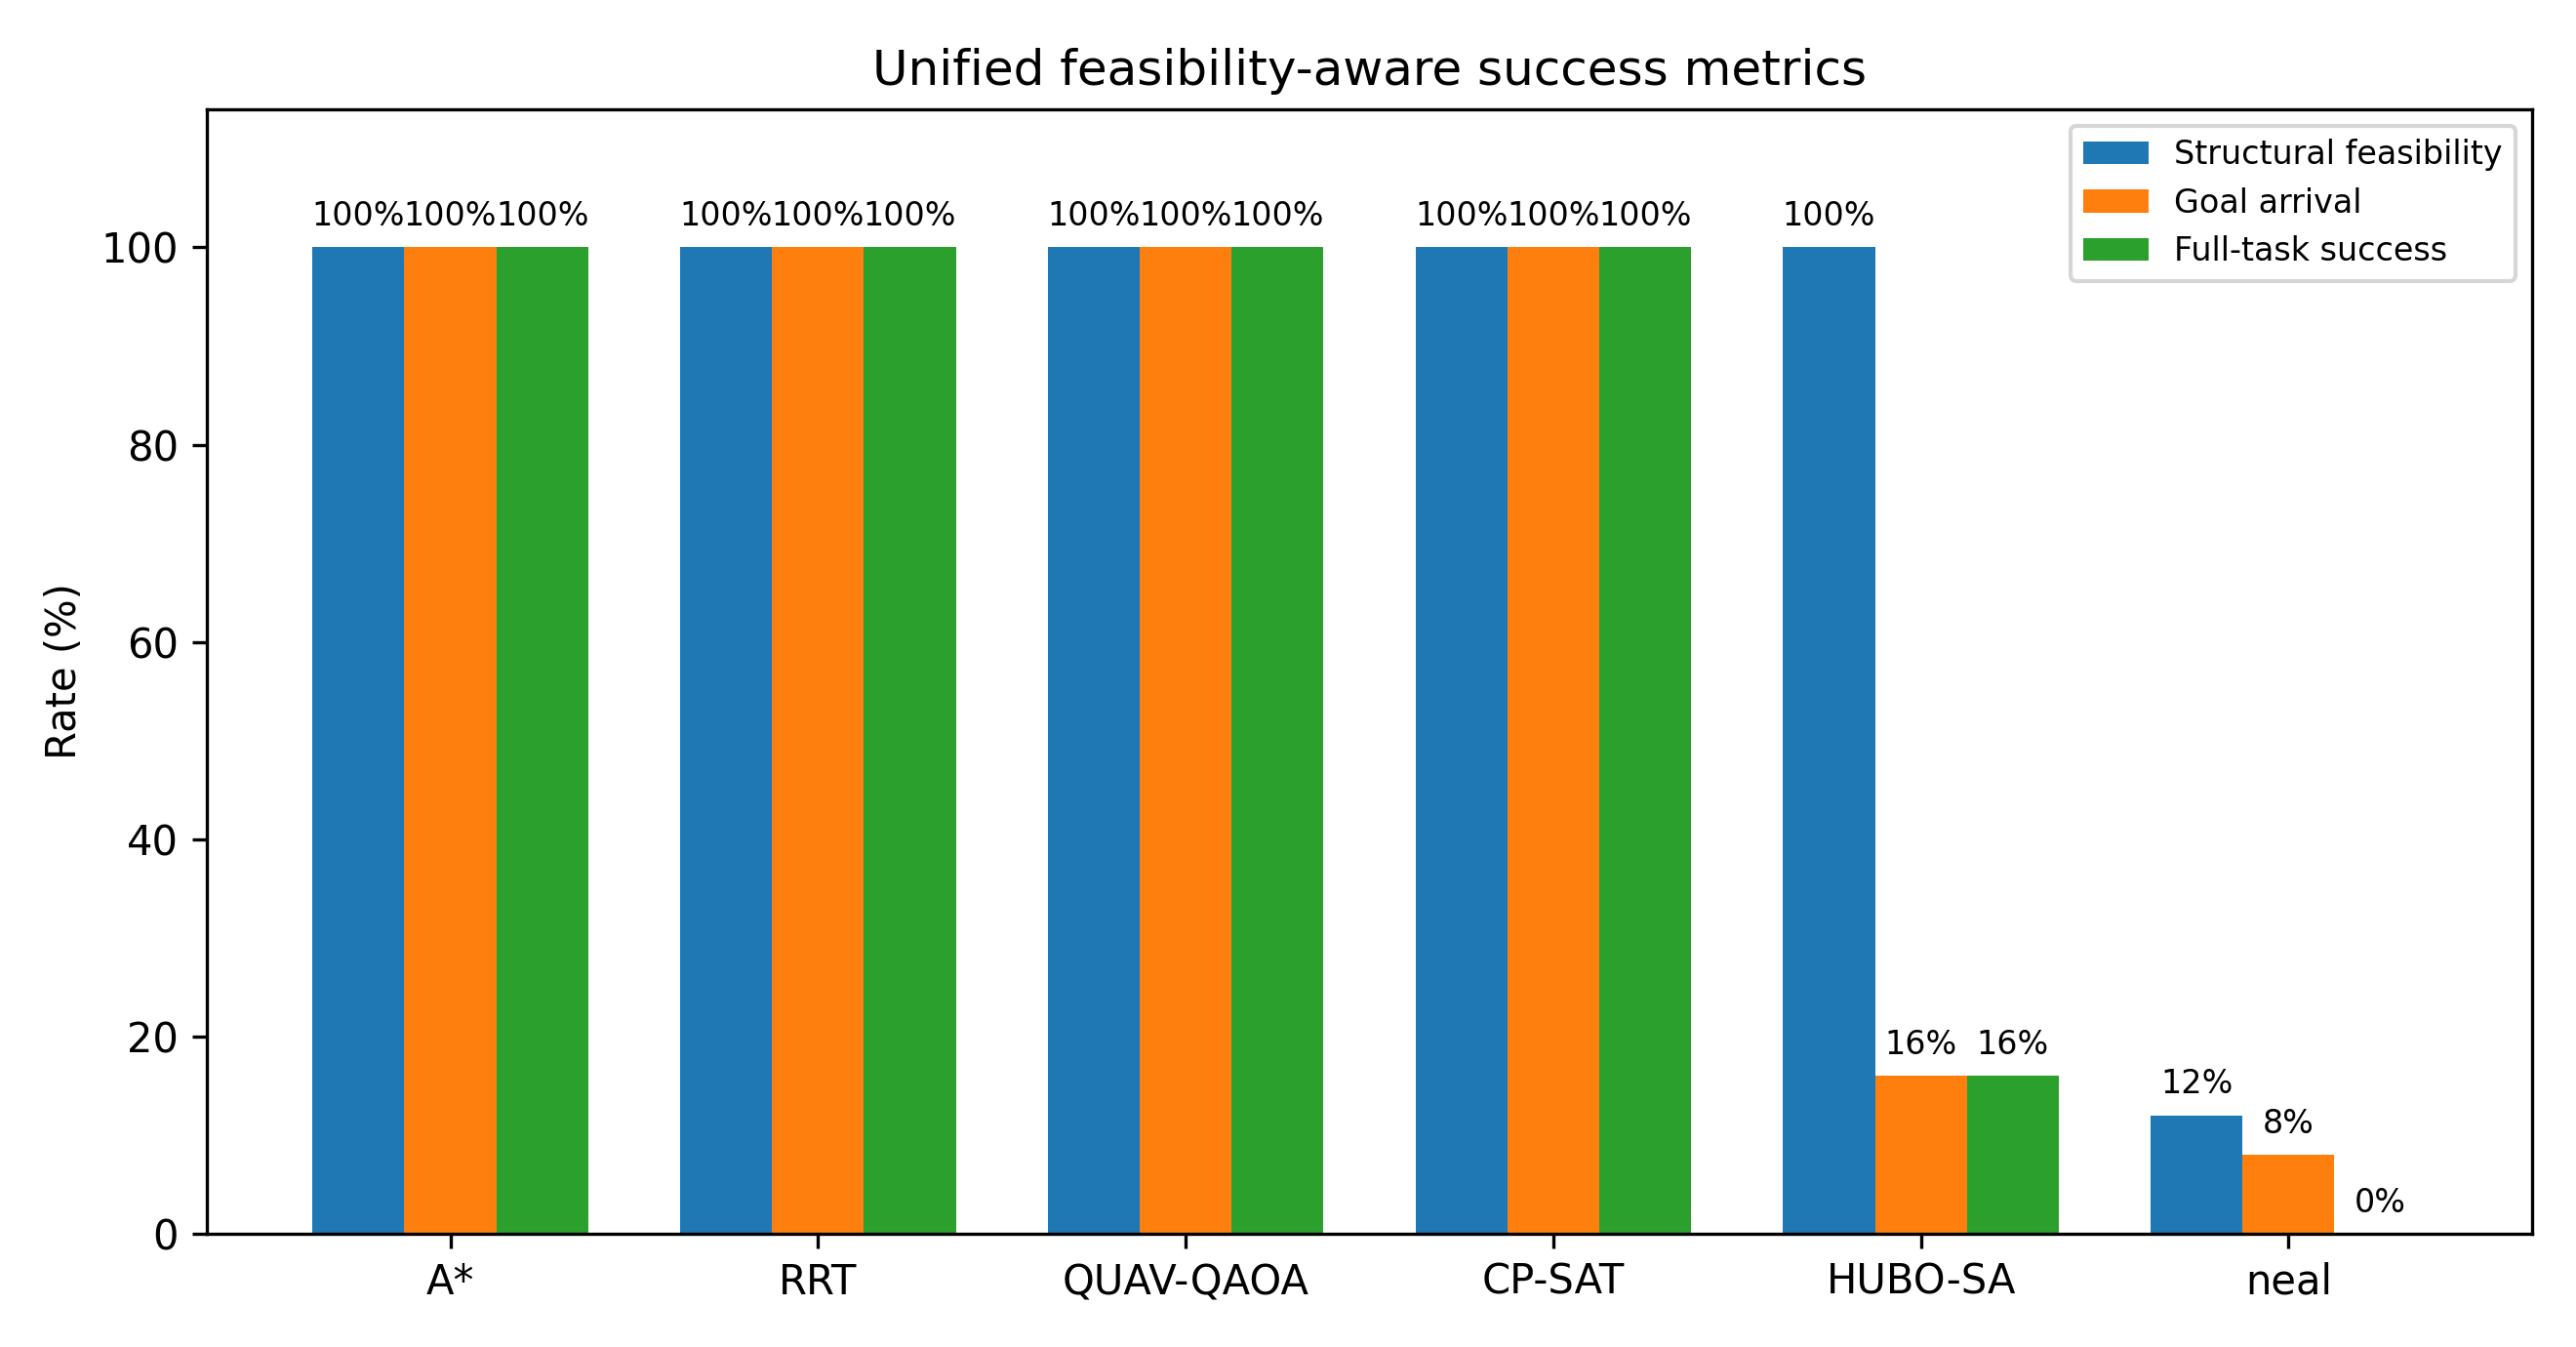
\includegraphics[width=0.98\linewidth]{fig_unified_success_with_cpsat.png}
\caption{Unified feasibility-aware success metrics. The exact CP-SAT run certifies a full-success optimum. \texttt{neal} has nonzero feasibility and goal-arrival rates separately, but zero full-task success.}
\label{fig:unified_success}
\end{figure}



\subsection{Penalty Sweep}
The penalty-weight sweep for \texttt{neal} shows that weak structural penalties permit low-energy but infeasible samples. In the updated run, structural feasibility was $0/15$ for $\lambda\in\{50,100,300,600\}$, $4/15$ at $\lambda=1000$, and $5/15$ at $\lambda=2000$. The best feasible soft cost improved from 915.4 to 590.6 between $\lambda=1000$ and $\lambda=2000$, still worse than A*, SA, and CP-SAT.

\FloatBarrier
\section{Discussion}
The results show why the paper's contribution is not a simple claim that quantum computing outperforms classical planning. On this instance, exact CP-SAT proves the optimum of the hard-feasible native-HUBO soft objective, A* is very fast, and trajectory-SA can find the exact optimum but with poor target-arrival reliability. The decoded paths in Fig.~\ref{fig:decoded_paths} make the solver differences explicit. The QUAV-style QAOA baseline is useful because it shows that a quantum-assisted geometric selector can produce a valid obstacle-free path on the same platform. However, the native HUBO objective distinguishes visibility, temporal buffer-risk, and terminal behavior in a different way. Therefore, same-platform decoded-path evaluation is necessary for fair comparison.

The exact CP-SAT/MILP formulation also clarifies the role of quantum-compatible solvers. If a QUBO sampler is used, it must overcome not only path planning but also one-hot, movement, obstacle, target, and quadratization constraints. The benchmark exposes these failure modes by reporting structural feasibility, goal arrival, and full-task success separately.

The QUAV-style row in Table~\ref{tab:unified} should be interpreted carefully: it is a candidate-path selector over generated paths, not a native solution of the full $x_{t,v}$ HUBO. This candidate-path route is practical because feasibility is mostly handled before optimization, but it optimizes over a restricted candidate set. Thus the quantum-compatible components demonstrate formulation and benchmarking pathways, not superiority over A*, CP-SAT, or MILP. Those classical methods remain the correctness anchors. If a quadratic sampler is used, the cubic term must first be reduced to quadratic form with auxiliary variables and additional penalties. This reduction is one of the benchmarked failure modes rather than a completed performance claim.

\section{Limitations and Future Work}
The model remains a grid abstraction without quadrotor dynamics, velocity, acceleration, heading, camera field-of-view dynamics, or continuous controls. The target is static, so the visibility term is linear; a moving-target or occlusion-free tracking formulation would require a separate derivation with time-varying target states and hard line-of-sight constraints. The QUAV-style baseline is not official QUAV code. Future work should study moving-target formulations, larger maps, stronger candidate-generation policies, and sensitivity of quadratization penalties.

\section{Conclusion}
This paper presents a feasibility-aware HUBO/QUBO benchmark and solver-analysis framework for UAV obstacle-avoidance with visibility cost. The higher-order structure comes from sustained temporal proximity to obstacle-buffer cells. The unified comparison with A*, RRT-best, QUAV-style QAOA, trajectory-SA, \texttt{neal}, and exact CP-SAT shows that geometric path quality, native HUBO energy, and full trajectory validity are different metrics. The CP-SAT run certifies the best observed SA path as optimal for the hard-feasible native-HUBO soft objective, while \texttt{neal} after quadratization has zero full-task success in the tested reads. The main contribution is therefore a rigorous quantum-compatible benchmark and feasibility-aware evaluation protocol, not a quantum-speedup claim.

\section*{Code Availability}
The code, figures, result logs, and benchmark implementations are available in the project repository~\cite{mohammadiGithub}: \url{https://github.com/alimohammadi44/uav-hubo-qiml-2026/tree/main}.

\begin{thebibliography}{99}
\bibitem{innan2025quav} N. Innan, M. Kashif, A. Marchisio, Y.-S. Gan, F. Barbaresco, and M. Shafique, ``QUAV: Quantum-assisted path planning and optimization for UAV navigation with obstacle avoidance,'' in \emph{Proc. IEEE Int. Conf. Quantum Artificial Intelligence (QAI)}, 2025, pp. 208--215, doi: 10.1109/QAI63978.2025.00040.
\bibitem{hart1968} P. E. Hart, N. J. Nilsson, and B. Raphael, ``A formal basis for the heuristic determination of minimum cost paths,'' \emph{IEEE Transactions on Systems Science and Cybernetics}, vol. 4, no. 2, pp. 100--107, 1968, doi: 10.1109/TSSC.1968.300136.
\bibitem{lavalle1998} S. M. LaValle, ``Rapidly-exploring random trees: A new tool for path planning,'' Tech. Rep. 98-11, Computer Science Dept., Iowa State University, Oct. 1998.
\bibitem{chen2016} J. Chen, T. Liu, and S. Shen, ``Tracking a moving target in cluttered environments using a quadrotor,'' in \emph{Proc. IEEE/RSJ Int. Conf. Intelligent Robots and Systems (IROS)}, 2016, pp. 446--453, doi: 10.1109/IROS.2016.7759092.
\bibitem{hausman2016} K. Hausman, G. Kahn, S. Patil, J. M\"uller, K. Goldberg, P. Abbeel, and G. S. Sukhatme, ``Occlusion-aware multi-robot 3D tracking,'' in \emph{Proc. IEEE/RSJ Int. Conf. Intelligent Robots and Systems (IROS)}, 2016, pp. 1863--1870, doi: 10.1109/IROS.2016.7759296.
\bibitem{penin2018} B. Penin, P. Robuffo Giordano, and F. Chaumette, ``Vision-based reactive planning for aggressive target tracking while avoiding collisions and occlusions,'' \emph{IEEE Robotics and Automation Letters}, vol. 3, no. 4, pp. 3725--3732, 2018, doi: 10.1109/LRA.2018.2856526.
\bibitem{falanga2018} D. Falanga, P. Foehn, P. Lu, and D. Scaramuzza, ``PAMPC: Perception-aware model predictive control for quadrotors,'' in \emph{Proc. IEEE/RSJ Int. Conf. Intelligent Robots and Systems (IROS)}, 2018, pp. 1--8, doi: 10.1109/IROS.2018.8593739.
\bibitem{wang2022} J. Wang, Y.-X. Wu, Y.-Q. Chen, and S. Ju, ``Multi-UAVs collaborative tracking of moving target with maximized visibility in urban environment,'' \emph{Journal of the Franklin Institute}, vol. 359, no. 11, pp. 5512--5532, 2022, doi: 10.1016/j.jfranklin.2022.05.004.
\bibitem{masnavi2022} H. Masnavi, V. K. Adajania, K. Kruusam\"ae, and A. K. Singh, ``Real-time multi-convex model predictive control for occlusion-free target tracking with quadrotors,'' \emph{IEEE Access}, vol. 10, pp. 29009--29031, 2022, doi: 10.1109/ACCESS.2022.3157977.
\bibitem{glover2019} F. Glover, G. Kochenberger, and Y. Du, ``Quantum bridge analytics I: A tutorial on formulating and using QUBO models,'' \emph{4OR}, vol. 17, no. 4, pp. 335--371, 2019, doi: 10.1007/s10288-019-00424-y.
\bibitem{farhi2014} E. Farhi, J. Goldstone, and S. Gutmann, ``A quantum approximate optimization algorithm,'' arXiv:1411.4028, 2014.
\bibitem{osaba2022review} E. Osaba, E. Villar-Rodriguez, and I. Oregi, ``A systematic literature review of quantum computing for routing problems,'' \emph{IEEE Access}, vol. 10, pp. 55805--55817, 2022, doi: 10.1109/ACCESS.2022.3177790.
\bibitem{huang2022} Z. Huang, Q. Li, J. Zhao, and M. Song, ``Variational quantum algorithm applied to collision avoidance of unmanned aerial vehicles,'' \emph{Entropy}, vol. 24, no. 11, Art. no. 1685, 2022, doi: 10.3390/e24111685.
\bibitem{davies2024} E. G. Davies and P. V. Kalidindi, ``Quantum algorithms for drone mission planning,'' in \emph{Proc. SPIE Quantum Technologies for Defence and Security}, vol. 13202, Art. no. 1320209, 2024, doi: 10.1117/12.3036340.
\bibitem{hua2024} R. Hua, D. Di Lorenzo, F. Chinesta, and P. Codognet, ``Quantum annealing solutions for drone route planning problems,'' in \emph{Proc. IEEE Int. Conf. Quantum Computing and Engineering (QCE)}, 2024, pp. 600--610, doi: 10.1109/QCE60285.2024.00076.
\bibitem{tarquini2026} S. Tarquini, D. Dragoni, M. Vandelli, and F. Tudisco, ``Testing quantum and simulated annealers on the drone delivery packing problem,'' \emph{Quantum Machine Intelligence}, vol. 8, Art. no. 14, 2026, doi: 10.1007/s42484-026-00362-z.
\bibitem{osaba2025q4dr} E. Osaba, P. Miranda-Rodriguez, A. Oikonomakis, M. Petri\v{c}, A. Ruiz, S. Bock, and M.-A. Kourtis, ``Solving drone routing problems with quantum computing: A hybrid approach combining quantum annealing and gate-based paradigms,'' in \emph{Proc. IEEE Congress on Evolutionary Computation (CEC)}, 2025, pp. 1--8, doi: 10.1109/CEC65147.2025.11042978.
\bibitem{qiu2025} G. Qiu, R. Lin, J. Zhu, and J. Ren, ``Quantum-driven UAV path planning using QUBO model and coherent Ising machines,'' in \emph{Proc. 8th Int. Conf. Advanced Algorithms and Control Engineering (ICAACE)}, 2025, pp. 388--393, doi: 10.1109/ICAACE65325.2025.11018976.
\bibitem{barbeau2025} M. Barbeau, F. Janabi-Sharifi, and H. Masnavi, ``A quantum annealing approach to target tracking,'' in \emph{Proc. IEEE Int. Conf. Robotics and Automation (ICRA)}, 2025, pp. 3022--3027, doi: 10.1109/ICRA55743.2025.11128357.
\bibitem{gerlach2025} T. Gerlach, L. K. Lee, F. Barbaresco, and N. Piatkowski, ``Hybrid quantum-classical multi-agent pathfinding,'' in \emph{Proc. 42nd Int. Conf. Machine Learning (ICML)}, ser. PMLR, vol. 267, pp. 19161--19171, 2025.
\bibitem{villasmil2026} J. Gonz\'alez Villasmil, ``Scalable multi-robot path planning via quadratic unconstrained binary optimization,'' arXiv:2602.14799, 2026, doi: 10.48550/arXiv.2602.14799.
\bibitem{neal} ``neal: Simulated annealing sampler for binary quadratic models,'' software package.
\bibitem{dimod} ``dimod: Binary quadratic model library,'' software package.
\bibitem{rosenberg1975} I. G. Rosenberg, ``Reduction of bivalent maximization to the quadratic case,'' \emph{Cahiers du Centre d'Etudes de Recherche Op\'erationnelle}, vol. 17, pp. 71--79, 1975.
\bibitem{ortools} L. Perron and V. Furnon, ``OR-Tools,'' Google, software package, \url{https://developers.google.com/optimization}.
\bibitem{mohammadiGithub} A. Mohammadi, ``UAV HUBO/QUBO benchmark,'' GitHub, 2026. [Online]. Available: \url{https://github.com/alimohammadi44/uav-hubo-qiml-2026/tree/main}.
\end{thebibliography}

\end{document}
